% TODO png blur? too wide listings
\mysection{Information avec l'entropie}
\label{entropy}
\myindex{Entropy}

\epigraph{Entropy: The quantitative measure of disorder, which in turn relates to the thermodynamic functions, temperature, and heat.}
{Dictionaire:  Applied Math for Engineers and Scientists}

Par soucis de simplification, je dirais que l'entropie est une mesure, d'à quel
point des données peuvent être compressées.
Par exemple, il est généralement impossible de compresser un fichier archive
déjà compressé, donc il a une entropie importante.
D'un autre coté, 1MiB d'octet à zéro peut être compressé en un tout petit fichier.
En effet, en français, un million de zéro peut être simplement décrit par
``le fichier résultant est un million d'octets à zéro''.
Les fichiers compressés sont en général une liste d'instructions destinées au dé-compresseur,
comme ceci:
``mettre 1000 zéros, puis l'octet 0x23, puis l'octet 0x45, puis un bloc d'une
taille de 10 octets que nous avons vu 500 octets avant, etc.''

Les textes écrits en langage naturel peuvent aussi être fortement compressés, car
le langage naturel a beaucoup de redondance (autrement, une petite typo conduirait
toujours à une incompréhension, comme un bit inversé dans un fichier archive rend
la décompression presque impossible), certains mots sont utilisés très souvent, etc.
Dans le discours courant, il est possible de supprimer jusqu'à la moitié
des mots et il est toujours compréhensible.

Le code pour les CPUs peut aussi être compressé, car certaines instructions \ac{ISA}
sont utilisées plus souvent que d'autres.
\myindex{x86!\Instructions!MOV}
\myindex{x86!\Instructions!PUSH}
\myindex{x86!\Instructions!CALL}
En x86, les instructions les plus utilisées sont \INS{MOV}/\INS{PUSH}/\INS{CALL}
(\myref{correctly_disasmed_code}).

La compression de données et le chiffrement tendent à produire des résultats avec
une très haute entropie.
Un bon \ac{PRNG} produit aussi des données qui ne peuvent pas être compressées
(il est possible de mesurer leur qualité par ce moyen).

Donc, autrement dit, la mesure de l'entropie peut aider à tester le contenu de bloc
de données inconnues.

\subsection{Analyse de l'entropie dans Mathematica}
\newcommand{\EntropyGfxScale}{0.8\textwidth}

(Cette partie est parue initialement sur mon blog le 13 mai 2015.
Quelques discussions: \url{https://news.ycombinator.com/item?id=9545276}.)

Il est possible de découper un fichier par blocs, de calculer l'entropie de chacun
d'eux et de dessiner un graphe.
J'ai fais ceci avec Wolfram Mathematica à titre de démonstration et voici le code
source (Mathematica 10):

\begin{lstlisting}[style=custommath]
(* loading the file *)
input=BinaryReadList["file.bin"];

(* setting block sizes *)
BlockSize=4096;BlockSizeToShow=256;

(* slice blocks by 4k *)
blocks=Partition[input,BlockSize];

(* how many blocks we've got? *)
Length[blocks]

(* calculate entropy for each block. 2 in Entropy[] (base) is set with the intention so Entropy[] 
function will produce the same results as Linux ent utility does *)
entropies=Map[N[Entropy[2,#]]&,blocks];

(* helper functions *)
fBlockToShow[input_,offset_]:=Take[input,{1+offset,1+offset+BlockSizeToShow}]
fToASCII[val_]:=FromCharacterCode[val,"PrintableASCII"]
fToHex[val_]:=IntegerString[val,16]
fPutASCIIWindow[data_]:=Framed[Grid[Partition[Map[fToASCII,data],16]]]
fPutHexWindow[data_]:=Framed[Grid[Partition[Map[fToHex,data],16],Alignment->Right]]

(* that will be the main knob here *)
{Slider[Dynamic[offset],{0,Length[input]-BlockSize,BlockSize}],Dynamic[BaseForm[offset,16]]}

(* main UI part *)
Dynamic[{ListLinePlot[entropies,GridLines->{{-1,offset/BlockSize,1}},Filling->Axis,AxesLabel->{"offset","entropy"}],
CurrentBlock=fBlockToShow[input,offset];
fPutHexWindow[CurrentBlock],
fPutASCIIWindow[CurrentBlock]}]
\end{lstlisting}

\subsubsection{Base de données GeoIP de FAI}

\myindex{GeoIP}
Commençons avec le fichier \href{https://www.maxmind.com/en/geoip-demo}{GeoIP} (qui
assigne un FAI au bloc d'adresses IP).
Ce fichier binaire \emph{GeoIPISP.dat} a plusieurs tables (qui sont peut-être les
intervalles d'adresses IP) plus quelques blobs de texte à la fin du fichier (contenant
les noms des FAI).

Lorsque je le charge dans Mathematica, je vois ceci:

\begin{figure}[H]
\centering
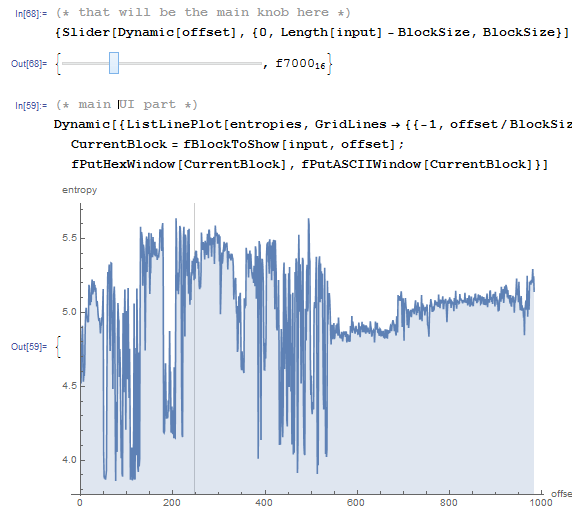
\includegraphics[width=\EntropyGfxScale]{ff/entropy/geoipisp11.png}
\end{figure}

\begin{figure}[H]
\centering
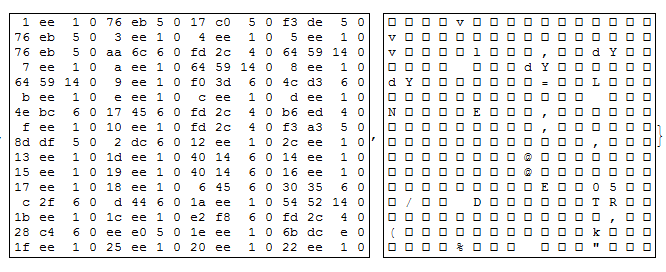
\includegraphics[width=\EntropyGfxScale]{ff/entropy/geoipisp12.png}
\end{figure}


Il y a deux parties dans le graphe: la première est un peu chaotique, la seconde
est plus régulière.

0 sur l'axe vertical du graphe signifie l'entropie la plus basse (les données
qui peuvent être compressée très fortement, \emph{ordonnées} en d'autres mots) et 8
est la plus haute (ne peuvent pas être compressées du tout, \emph{chaotique}
ou \emph{aléatoires} en d'autres mots).
Pourquoi 0 et par 8? 0 signifie 0 bits par octet (l'octet en tant que conteneur
n'est pas rempli du tout) et 8 signifie 8 bits par octet, i.e., l'octet comme
conteneur est complètement rempli d'information.

Donc, je mets le curseur pour pointer sur le milieu du premier bloc, et je vois clairement
des tableaux d'entiers 32-bit.
Maintenant je mets le curseur au milieu du second bloc et je vois un texte en anglais:

\begin{figure}[H]
\centering
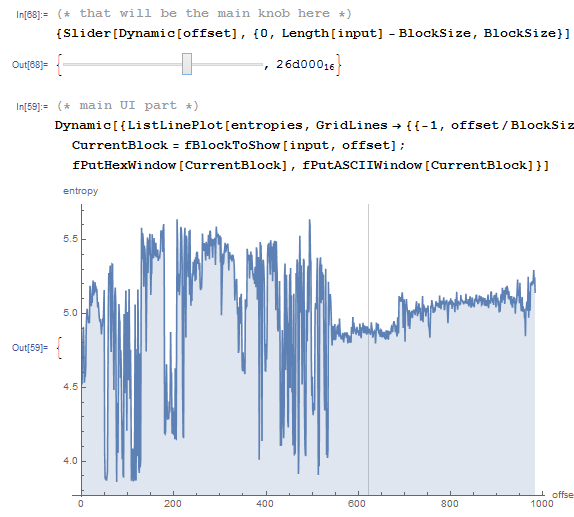
\includegraphics[width=\EntropyGfxScale]{ff/entropy/geoipisp21.png}
\end{figure}

\begin{figure}[H]
\centering
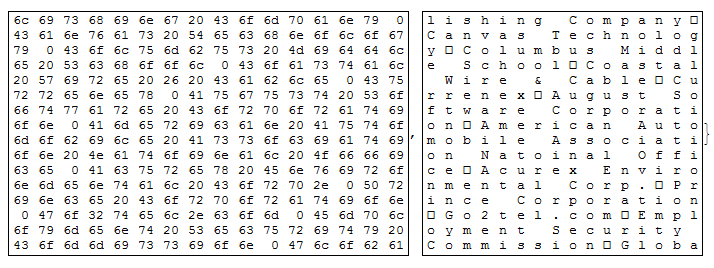
\includegraphics[width=\EntropyGfxScale]{ff/entropy/geoipisp22.png}
\end{figure}


En effet, ceci sont les noms des FAIs.
Donc, l'entropie de textes en anglais est 4.5-5 bits par octet? Oui, quelque chose
comme ça.
Wolfram Mathematica comprend quelques corpus de littérature anglaise bien connu,
et nous pouvons voir l'entropie de sonnets de Shakespeare:

\begin{lstlisting}[style=custommath]
In[]:= Entropy[2,ExampleData[{"Text","ShakespearesSonnets"}]]//N
Out[]= 4.42366
\end{lstlisting}

4,4 est proche de ce que nous obtenons ()4.7-5.3).
Bien sûr, les textes de la littérature anglaise classique sont quelques peu différents
des noms des FAIs et autres texte en anglais que nous pouvons trouver dans des fichiers
binaires (débogage/trace/messages d'erreur), mais cette valeur est proche.

\subsubsection{Firmware TP-Link WR941 }

Pour l'exemple suivant, j'ai pris le firmware du routeur TP-Link WR941:

\begin{figure}[H]
\centering
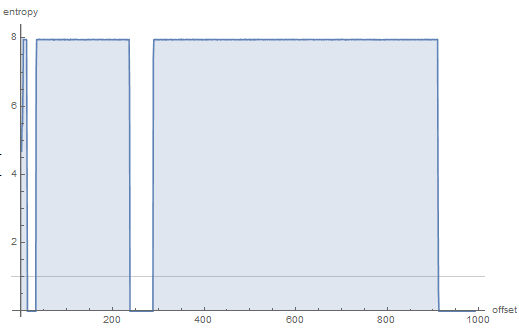
\includegraphics[width=\EntropyGfxScale]{ff/entropy/tplink.png}
\end{figure}


Nous voyons ici 3 blocs avec des vides.
Puis le premier bloc avec une haute entropie (démarrant à l'adresse 0) est petit,
le second (adresse quelque part en 0x22000) et plus grand et le troisième
(adresse 0x123000) est le plus grand.
Je ne peux pas être certain de l'entropie du premier bloc, mais le 2-ème et le 3-ème
ont une entropie très haute, signifiant que ces blocs sont soit compressés et/ou
chiffrés.

\myindex{Binwalk}
J'ai essayé \href{http://binwalk.org/}{binwalk} pour ce fichier de firmware:

\begin{lstlisting}
DECIMAL       HEXADECIMAL     DESCRIPTION
--------------------------------------------------------------------------------
0             0x0             TP-Link firmware header, firmware version: 0.-15221.3, image version: "", product ID: 0x0, product version: 155254789, kernel load address: 0x0, kernel entry point: 0x-7FFFE000, kernel offset: 4063744, kernel length: 512, rootfs offset: 837431, rootfs length: 1048576, bootloader offset: 2883584, bootloader length: 0
14832         0x39F0          U-Boot version string, "U-Boot 1.1.4 (Jun 27 2014 - 14:56:49)"
14880         0x3A20          CRC32 polynomial table, big endian
16176         0x3F30          uImage header, header size: 64 bytes, header CRC: 0x3AC66E95, created: 2014-06-27 06:56:50, image size: 34587 bytes, Data Address: 0x80010000, Entry Point: 0x80010000, data CRC: 0xDF2DBA0B, OS: Linux, CPU: MIPS, image type: Firmware Image, compression type: lzma, image name: "u-boot image"
16240         0x3F70          LZMA compressed data, properties: 0x5D, dictionary size: 33554432 bytes, uncompressed size: 90000 bytes
131584        0x20200         TP-Link firmware header, firmware version: 0.0.3, image version: "", product ID: 0x0, product version: 155254789, kernel load address: 0x0, kernel entry point: 0x-7FFFE000, kernel offset: 3932160, kernel length: 512, rootfs offset: 837431, rootfs length: 1048576, bootloader offset: 2883584, bootloader length: 0
132096        0x20400         LZMA compressed data, properties: 0x5D, dictionary size: 33554432 bytes, uncompressed size: 2388212 bytes
1180160       0x120200        Squashfs filesystem, little endian, version 4.0, compression:lzma, size: 2548511 bytes, 536 inodes, blocksize: 131072 bytes, created: 2014-06-27 07:06:52
\end{lstlisting}

\myindex{LZMA}
En effet: il y a des choses au début, mais deux larges blocs compressés LZMA
commencent en 0x20400 et 0x120200.
Ce sont en gros les adresses que nous avons vu dans Mathematica.
Oh, à propos, binwalk peut aussi afficher l'entropie (option \TT{-E}):

\begin{lstlisting}
DECIMAL       HEXADECIMAL     ENTROPY
--------------------------------------------------------------------------------
0             0x0             Falling entropy edge (0.419187)
16384         0x4000          Rising entropy edge (0.988639)
51200         0xC800          Falling entropy edge (0.000000)
133120        0x20800         Rising entropy edge (0.987596)
968704        0xEC800         Falling entropy edge (0.508720)
1181696       0x120800        Rising entropy edge (0.989615)
3727360       0x38E000        Falling entropy edge (0.732390)
\end{lstlisting}

Les fronts ascendants correspondent à des fronts ascendants de blocs sur notre graphe.
Les fronts descendants sont des points où des espaces vides commencent.

Binwalk peut aussi générer un graphe PNG (\TT{-E -J}):

\begin{figure}[H]
\centering
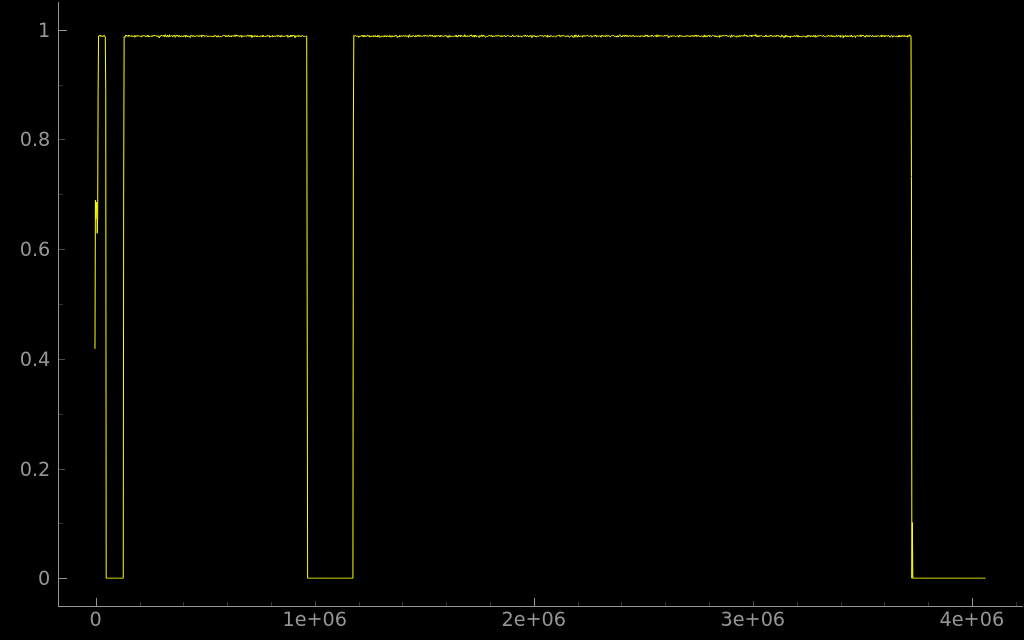
\includegraphics[width=\EntropyGfxScale]{ff/entropy/tplink_binwalk.png}
\end{figure}


Que pouvons-nous dire à propos de ces espaces vides? En regardant dans un éditeur hexadécimal,
nous voyons qu'ils sont simplement remplis avec des octets à 0xFF.
Pourquoi les développeurs les ont-ils mises?
Peut-être parce qu'ils n'ont pas pu calculer précisément la taille des blocs compressés,
et leurs ont donc alloué de l'espace avec une marge.

\subsubsection{Notepad}

\myindex{Notepad}

Un autre exemple est notepad.exe que j'ai pris dans Windows 8.1:

\begin{figure}[H]
\centering
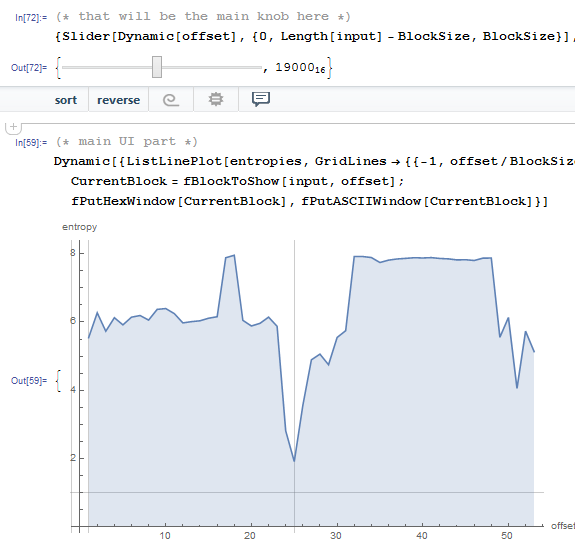
\includegraphics[width=\EntropyGfxScale]{ff/entropy/notepad11.png}
\end{figure}

\begin{figure}[H]
\centering
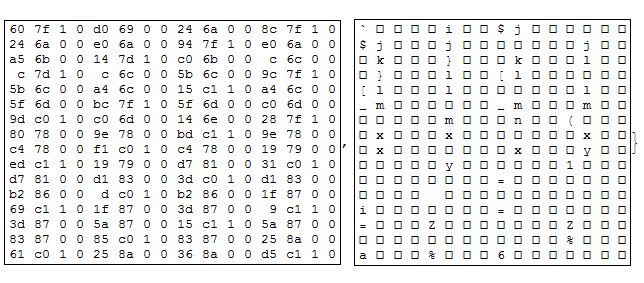
\includegraphics[width=\EntropyGfxScale]{ff/entropy/notepad12.png}
\end{figure}


Il y a un creux à $\approx 0x19000$ (offset absolu dans le fichier).
J'ai ouvert le fichier exécutable dans un éditeur hexadécimal et trouvé des tables
d'imports (qui ont une entropie plus basse que le code x86-64 dans la première moitié
du graphe).

Il y a aussi un bloc avec une grande entropie qui démarre $\approx 0x20000$:

\begin{figure}[H]
\centering
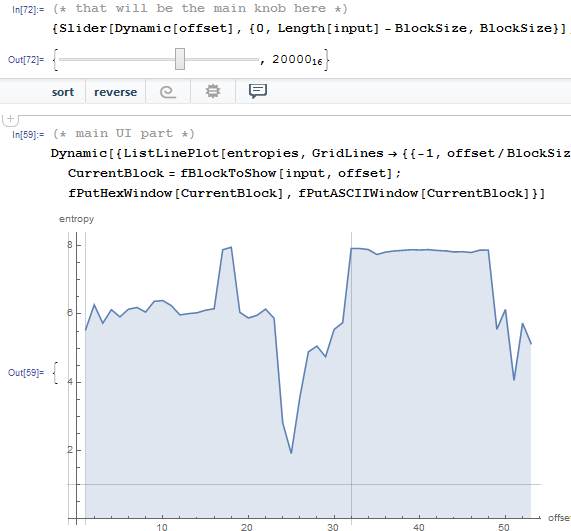
\includegraphics[width=\EntropyGfxScale]{ff/entropy/notepad21.png}
\end{figure}

\begin{figure}[H]
\centering
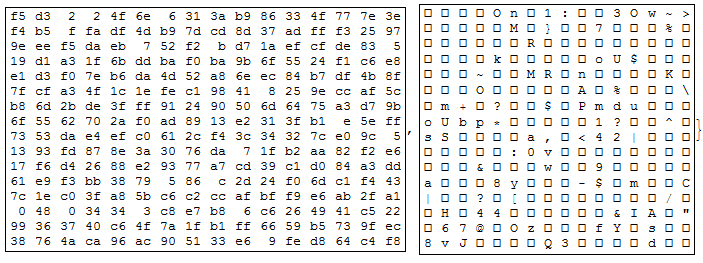
\includegraphics[width=\EntropyGfxScale]{ff/entropy/notepad22.png}
\end{figure}


\myindex{PNG}
Dans un éditeur hexadécimal je peux y voir un fichier PNG, inséré dans la section
ressource du fichier PE (c'est une grosse image de l'icône de notepad).
Les fichiers PNG sont compressés, en effet.

\subsubsection{Dashcam sans marque}

Maintenant l'exemple le plus avancé dans cette partie est le firmware d'une dashcam
sans marque que j'ai reçu d'un ami:

\begin{figure}[H]
\centering
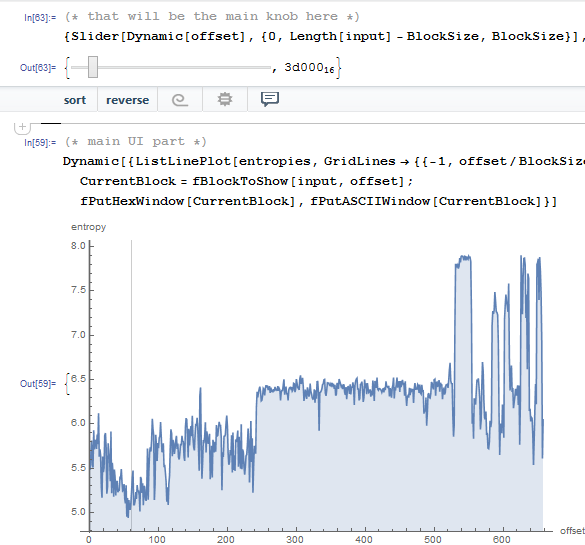
\includegraphics[width=\EntropyGfxScale]{ff/entropy/dashcam_text1.png}
\end{figure}

\begin{figure}[H]
\centering
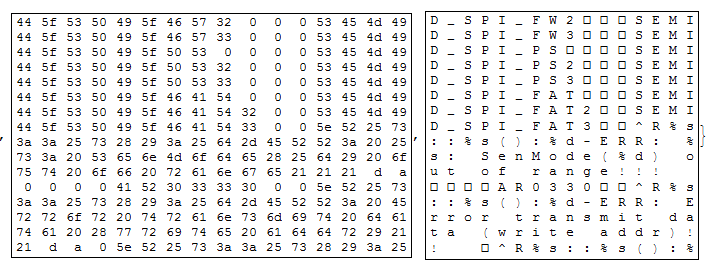
\includegraphics[width=\EntropyGfxScale]{ff/entropy/dashcam_text2.png}
\end{figure}


La creux au tout début est un texte en anglais: messages de débogage.
\myindex{MIPS}
J'ai vérifié différents \ac{ISA}s et j'ai trouvé que le premier tiers du fichier
complet (avec le segment de texte dedans) est en fait du code MIPS (petit-boutiste).

Par exemple, ceci est une fonction épilogue MIPS très typique:

\begin{lstlisting}[style=customasmMIPS]
ROM:000013B0                 move    $sp, $fp
ROM:000013B4                 lw      $ra, 0x1C($sp)
ROM:000013B8                 lw      $fp, 0x18($sp)
ROM:000013BC                 lw      $s1, 0x14($sp)
ROM:000013C0                 lw      $s0, 0x10($sp)
ROM:000013C4                 jr      $ra
ROM:000013C8                 addiu   $sp, 0x20
\end{lstlisting}

D'après notre graphe nous pouvons voir que le code MIPs a une entropie de 5-6 bits
par octet.
En effet, j'ai mesuré une fois l'entropie de différents \ac{ISA}s et j'ai obtenu
ces valeurs:

\begin{itemize}
\item x86: section .text du fichier ntoskrnl.exe de Windows 2003: 6.6
\item x64: section .text du fichier ntoskrnl.exe de Windows 7 x64: 6.5
\item ARM (mode thumb), Angry Birds Classic: 7.05
\item ARM (mode ARM) Linux Kernel 3.8.0: 6.03
\item MIPS (little endian), section .text du fichier user32.dll de Windows NT 4: 6.09
\end{itemize}

Donc l'entropie du code exécutable est plus grande que du texte en anglais, mais
peut encore être compressé.

Maintenant le second tiers qui commence en 0xF5000. Je ne sais pas ce que c'est.
J'ai essayé différents \ac{ISA}s mais sans succès.
L'entropie de ce bloc semble encore plus régulière que celui de l'exécutable.
Peut-être des sortes de données?

\myindex{JPEG}
Il y a aussi un pic en $\approx 0x213000$.
Je l'ai vérifié dans un éditeur hexadécimal et j'y ai trouvé un fichier JPEG (qui
est, bien sûr, compressé)!
Je ne sais pas ce qu'il y a à la fin.
Essayons Binwalk pour ce fichier:

\begin{lstlisting}
% binwalk FW96650A.bin 

DECIMAL       HEXADECIMAL     DESCRIPTION
--------------------------------------------------------------------------------
167698        0x28F12         Unix path: /15/20/24/25/30/60/120/240fps can be served..
280286        0x446DE         Copyright string: "Copyright (c) 2012 Novatek Microelectronic Corp."
2169199       0x21196F        JPEG image data, JFIF standard 1.01
2300847       0x231BAF        MySQL MISAM compressed data file Version 3

% binwalk -E FW96650A.bin 

DECIMAL       HEXADECIMAL     ENTROPY
--------------------------------------------------------------------------------
0             0x0             Falling entropy edge (0.579792)
2170880       0x212000        Rising entropy edge (0.967373)
2267136       0x229800        Falling entropy edge (0.802974)
2426880       0x250800        Falling entropy edge (0.846639)
2490368       0x260000        Falling entropy edge (0.849804)
2560000       0x271000        Rising entropy edge (0.974340)
2574336       0x274800        Rising entropy edge (0.970958)
2588672       0x278000        Falling entropy edge (0.763507)
2592768       0x279000        Rising entropy edge (0.951883)
2596864       0x27A000        Falling entropy edge (0.712814)
2600960       0x27B000        Rising entropy edge (0.968167)
2607104       0x27C800        Rising entropy edge (0.958582)
2609152       0x27D000        Falling entropy edge (0.760989)
2654208       0x288000        Rising entropy edge (0.954127)
2670592       0x28C000        Rising entropy edge (0.967883)
2676736       0x28D800        Rising entropy edge (0.975779)
2684928       0x28F800        Falling entropy edge (0.744369)
\end{lstlisting}

Oui, il trouve un fichier JPEG et même des données MySQL!
Mais je ne suis pas certain que ça soit vrai---je ne l'ai pas encore vérifié.

\myindex{clusterization}
Il est aussi intéressant d'essayer la clusterisation dans Mathematica:

\begin{figure}[H]
\centering
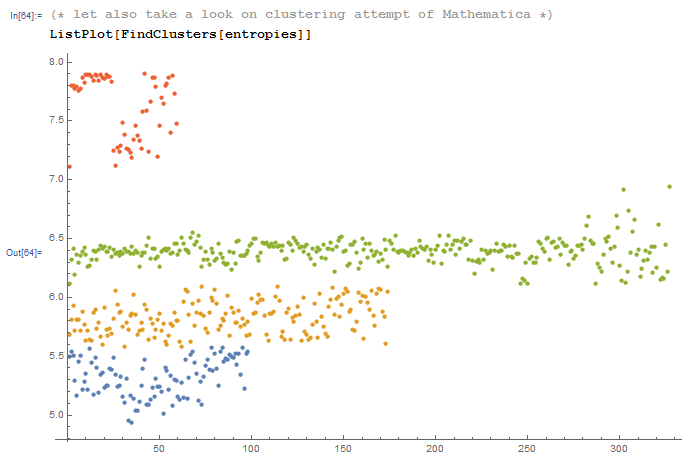
\includegraphics[width=\EntropyGfxScale]{ff/entropy/dashcam_clusters.png}
\end{figure}


Ceci est un exemple de la façon dont Mathematica groupe des valeurs d'entropie diverses
dans des groupes distincts.
En effet, c'est quelque chose de plausible.
Les points bleus dans l'intervalle 5.0-5.5 sont probablement relatif à du texte en
anglais,
Les points jaunes dans 5.5-6 sont du code MIPS. Beaucoup de points verts dans 6.0-6.5
sont dans le second tiers non identifié.
Les points orange proches de 8.0 sont relatifs au fichier JPEG compressé.
D'autres points orange sont probablement relatif à la fin du firmware (données inconnues
pour nous).

\subsubsection{Liens}

Fichiers binaires utilisés dans cette partie: \\
\url{\RepoURL/ff/entropy/files/}.\\
Fichier notebook Wolfram Mathematica: \\
\url{\RepoURL/ff/entropy/files/binary_file_entropy.nb} \\
(toutes les cellules doivent être évaluées pour que ça commence à fonctionner).


\subsection{Conclusion}

L'entropie peut-être utilisée comme un moyen rapide d'investigation de fichiers inconnus.
En particulier, c'est un moyen rapide de trouver des morceaux de données compressées/chiffrées.
Quelqu'un a dit qu'il est possible de trouver des clefs \ac{RSA} privées/publiques
(et d'autres algorithmes cryptographiques) dans du code exécutable (les clefs ont
aussi une très grande entropie), mais je n'ai pas essayé moi-même.

\subsection{Outils}

L'utilitaire Linux \emph{ent} est très pratique pour trouver l'entropie d'un
fichier\footnote{\url{http://www.fourmilab.ch/random/}}.

Il y a un excellent visualiseur d'entropie en ligne fait par Aldo Cortesi,
que j'ai essayé d'imiter avec Mathematica: \url{http://binvis.io}.
Ses articles sur l'entropie valent la peine d'être lus:
\url{http://corte.si/posts/visualisation/entropy/index.html},
\url{http://corte.si/posts/visualisation/malware/index.html},
\url{http://corte.si/posts/visualisation/binvis/index.html}.

\myindex{radare2}
Le quadriciel radare2 a la commande \emph{\#entropy} pour ceci.

Un outil pour IDA: IDAtropy\footnote{\url{https://github.com/danigargu/IDAtropy}}.

\subsection{Un mot à propos des primitives de chiffrement comme le XORage}

Il est intéressant de noter que le chiffrement par un simple XOR n'affecte pas
l'entropie des données.
J'ai montré ceci dans l'exemple \emph{Norton Guide} de ce livre (\myref{norton_guide}).

Généralisation: le chiffrement par substitution n'affecte pas l'entropie des données
(et XOR peut être vu comme un chiffrement par substitution).
La raison est que l'algorithme de calcul de l'entropie voit les données au niveau
de l'octet.
D'un autre côté, les données chiffrées par un pattern XOR de 2 ou 4 octets donnent
un autre niveau d'entropie.

Néanmoins, une entropie basse est en général un signe de chiffrement amateur faible
(qui est aussi utilisé dans les clefs/fichiers de licence, etc.).

\subsection{Plus sur l'entropie de code exécutable}

Il est rapidement perceptible que la plus grande source d'entropie dans du code
exécutable est probablement dûe aux offsets encodés dans les opcodes.
Par exemple, ces deux instructions consécutives vont avoir des offsets relatifs
différents dans leur opcode, alors qu'elles pointent en fait sur la même fonction:

\begin{lstlisting}[style=customasmx86]
function proc
...
function endp

...

CALL function
...
CALL function
\end{lstlisting}

Un compresseur de code exécutable idéal encoderait l'information comme ceci:
\emph{Il y a un CALL à ``function'' à l'adresse X et la même CALL à l'adresse Y}
sans nécessiter d'encoder deux fois l'adresse de \emph{function}.

\myindex{UPX}
Pour gérer ceci, les compresseurs de code exécutable sont parfois capable de réduire
l'entropie ici.
Un exemple est UPX: \url{http://sourceforge.net/p/upx/code/ci/default/tree/doc/filter.txt}.

\subsection{\ac{PRNG}}

\myindex{GnuPG}
Lorsque je lance GnuPG pour générer une nouvelle clef privée (secrète), il demande
de l'entropie \dots

\begin{lstlisting}
We need to generate a lot of random bytes. It is a good idea to perform
some other action (type on the keyboard, move the mouse, utilize the
disks) during the prime generation; this gives the random number
generator a better chance to gain enough entropy.

Not enough random bytes available.  Please do some other work to give
the OS a chance to collect more entropy! (Need 169 more bytes)
\end{lstlisting}

Ceci signifie qu'un bon \ac{PRNG} prend longtemps pour produire des résultats avec
une haute entropie, et ceci est ce dont la clef cryptographique secrète à besoin.
Mais un \ac{CPRNG} est compliqué (car un ordinateur est lui-même un dispositif
hautement déterministe), donc GnuPG demande du hasard supplémentaire à l'utilisateur.

\subsection{Plus d'exemples}

Voici un cas où j'ai essayé de calculer l'entropie de certains blocs avec du
contenu inconnu: \myref{encrypted_DB1}.

\subsection{Entropie de fichiers variés}

L'entropie de données aléatoires est proche de 8:

\begin{lstlisting}
% dd bs=1M count=1 if=/dev/urandom | ent
Entropy = 7.999803 bits per byte.
\end{lstlisting}

Ceci signifie que presque tout l'espace disponible d'un octet est rempli d'information.

256 octets répartis dans l'intervalle 0..255 donnent exactement une valeur de 8:

\begin{lstlisting}[style=custompy]
#!/usr/bin/env python
import sys

for i in range(256):
    sys.stdout.write(chr(i))
\end{lstlisting}

\begin{lstlisting}
% python 1.py | ent
Entropy = 8.000000 bits per byte.
\end{lstlisting}

L'ordre des octets est sans importance.
Ceci signifie que tout l'espace dans un octet est rempli.

L'entropie de tout bloc rempli d'octets à zéro est 0:

\begin{lstlisting}
% dd bs=1M count=1 if=/dev/zero | ent
Entropy = 0.000000 bits per byte.
\end{lstlisting}

L'entropie d'une chaîne constituée d'un seul (n'importe lequel) octet est 0:

\begin{lstlisting}
% echo -n "aaaaaaaaaaaaaaaaaaa" | ent
Entropy = 0.000000 bits per byte.
\end{lstlisting}

\myindex{base64}
L'entropie d'une chaîne en base64 est la même que la données source, mais multiplié
par $\frac{3}{4}$.
Ceci car l'encodage base64 utilise 64 symboles au lieu de 256.

\begin{lstlisting}
% dd bs=1M count=1 if=/dev/urandom | base64 | ent
Entropy = 6.022068 bits per byte.
\end{lstlisting}

Peut-être que 6.02, assez proche de 6, est dû au caractère de remplissage (\TT{=}) qui
fausse un peu nos statistiques.

\myindex{Uuencode}
Uuencode utilise aussi 64 symboles:

\begin{lstlisting}
% dd bs=1M count=1 if=/dev/urandom | uuencode - | ent
Entropy = 6.013162 bits per byte.
\end{lstlisting}

Ceci signifie que les chaînes base64 et Uuencode peuvent être transmises en utilisant
des octets ou caractères sur 6-bit.

Toute information aléatoire au format hexadécimal a une entropie de 4 bits par octet:

\begin{lstlisting}
% openssl rand -hex $\$$(( 2**16 )) | ent
Entropy = 4.000013 bits per byte.
\end{lstlisting}

L'entropie d'un texte en anglais pris au hasard dans la bibliothèque Gutenbert a
une entropie de $\approx 4.5$.
La raison de ceci est que les textes anglais utilisent principalement 26 symboles,
et $log_2(26)=\approx 4.7$, i.e., vous aurez besoin d'octets de 5-bit pour transmettre
des textes en anglais non compressés, ça sera suffisant (ça l'était en effet au temps
du télétype).

Le texte choisi au hasard dans la bibliothèque \url{http://lib.ru} est l'``Idiot''\footnote{\url{http://az.lib.ru/d/dostoewskij_f_m/text_0070.shtml}},
de F.M.Dostoevsky qui est encodé en CP1251.

Et ce fichier a une entropie de $\approx 4.98$.
Le russe comporte 33 caractères et $log_2(33)=\approx 5.04$.
Mais il le caractère ``ё'' est impopulaire et rare.
% FIXME YO letter isn't rendered in Eng version
Et $log_2(32)=5$ (l'alphabet russe sans ce caractère rare)---maintenant ceci est
proche de ce que nous avons obtenu.

Quoiqu'il en soit, le texte dont nous parlons utilise la lettre ``ё', mais, sans
doute y est-elle rarement utilisée.

\myindex{UTF-8}
Le même fichier transcodé de CP1251 en UTF-8 donne une entropie de $\approx 4.23$.
Chaque caractère cyrillique encodé en UTF-8 est généralement encodé en une paire,
et le premier octet est toujours: 0xD0 ou 0xD1.
C'est peut-être ce qui cause ce biais.

Générons des bits aléatoirement et écrivons les avec les caractères ``T'' et ``F'':

\begin{lstlisting}[style=custompy]
#!/usr/bin/env python
import random, sys

rt=""
for i in range(102400):
    if random.randint(0,1)==1:
        rt=rt+"T"
    else:
        rt=rt+"F"
print rt
\end{lstlisting}

Échantillon: \TT{...TTTFTFTTTFFFTTTFTTTTTTFTTFFTTTFTFTTFTTFFFFFF...}.

L'entropie est très proche de 1 (i.e., 1 bit par octet).

Générons des chiffres décimaux aléatoirement:

\begin{lstlisting}[style=custompy]
#!/usr/bin/env python
import random, sys

rt=""
for i in range(102400):
    rt=rt+"%d" % random.randint(0,9)
print rt
\end{lstlisting}

Échantillon: \TT{...52203466119390328807552582367031963888032...}.

L'entropie sera proche de 3.32, en effet, c'est $log_2(10)$.


\subsection{Réduire le niveau d'entropie}

J'ai vu une fois un logiciel qui stockait chaque octet de données chiffrées sur 3 octets:
chacun avait une valeur de {\Large $\approx \frac{byte}{3}$}, donc reconstruire
l'octet chiffré impliquait de faire la somme de 3 octets consécutifs.
Ça semble absurde.

Mais certaines personnes disent que ça a été fait pour pour cacher le fait que les
données contenaient quelque chose de chiffré: la mesure de l'entropie d'un tel bloc
donnait une valeur bien plus faible.

